\documentclass{llncs}

\usepackage{hyperref}

\usepackage{amsmath}
\usepackage{stmaryrd}
\usepackage{amssymb}
\usepackage{float}

\def\Po#1#2{\Pos_{#1}{(#2)}}
\def\regw#1{\Reg{(#1)}}
\DeclareMathOperator{\Reg}{RegExp}
\DeclareMathOperator{\E}{E}
\DeclareMathOperator{\h}{H}
\DeclareMathOperator{\f}{F}
\DeclareMathOperator{\G}{G}
\DeclareMathOperator{\First}{First}
\DeclareMathOperator{\Follow}{Follow}
\DeclareMathOperator{\rooot}{root}
\DeclareMathOperator{\Pos}{Pos}
\def\b#1{\overline{#1}}

\usepackage{tikz}
\usetikzlibrary{automata}
\usetikzlibrary{shadows}

\usetikzlibrary{arrows}
\usetikzlibrary{shapes}
\usetikzlibrary{decorations.pathmorphing}
\usetikzlibrary{fit}
\tikzstyle{every picture}=[>=stealth',shorten >=1pt,node distance=1.44cm,bend angle=45,initial text=,every state/.style={inner sep=0.75mm, minimum size=1mm},font=\scriptsize]

\addtolength{\intextsep}{-7mm}

\pagestyle{plain}

\begin{document}

\title{An Efficient Algorithm for the Equation Tree Automaton \emph{via} the -C-Continuations}
\author{Ludovic Mignot, Nadia Ouali Sebti and Djelloul Ziadi  \thanks{\email{\{ludovic.mignot, nadia.ouali-sebti, djelloul.ziadi\}@univ-rouen.fr}}}
\institute{Laboratoire LITIS - EA 4108 Universit\'e de Rouen, Avenue de l'Universit\'e \\76801 Saint-\'Etienne-du-Rouvray Cedex.}



\maketitle

\begin{abstract}
  Champarnaud and Ziadi, and Khorsi \emph{et al.} show how to compute the equation automaton of word regular expression  \emph{via} the -C-Continuations.
  Kuske and Meinecke extend the computation of the equation automaton to a regular tree expression  over a ranked alphabet  and produce a  time and space complexity algorithm, where  is the maximal rank of a symbol  occurring  in  and  is the size of . In this paper, we give a full description of the algorithm based on the acyclic minimization of Revuz. Our algorithm, which is performed in an  time and space complexity, where  is the number of states of the produced automaton, is more efficient than the one obtained by Kuske and Meinecke.
\end{abstract}

\section{Introduction}

Regular expressions, which are finite representatives of potentially infinite languages, are widely used in various application areas such as XML Schema Languages~\cite{xml}, logic and verification~\cite{verif}, \emph{etc.} The concept of word regular expressions  has been extended to tree regular expressions. Similarly to word expressions, one can convert them into  finite recognizers, the tree automata.
 
 The study of the different  ways of conversion of regular expressions into automata and \emph{vice versa} is a very  active  field. There exists a lot  of techniques to transform regular expressions (resp. regular tree expressions)  into finite automata~\cite{Brug,glushkov,khorsi,ZPC} (resp. into finite tree automata~\cite{automate2,lata}). As far as tree automata are concerned, computation algorithms are extensions of word cases. In~\cite{lata}, the computation of the position tree automaton from  a regular tree expression has been achieved by extending the classical notions of Glushkov functions defined  in~\cite{glushkov}, leading to the computation of an automaton which number of states is linear w.r.t. the number of  occurrences of symbols but which number of transitions can be exponential. In the same paper, it is proved that this automaton can be reduced  into a quadratic size recognizer.
 
 On the other side, Kuske and Meinecke have extended the notion of  word partial derivatives~\cite{antimirov} into  tree partial derivatives. They also present how to compute them extending  from words to trees~\cite{automate2} the -C-Continuation algorithm by Champarnaud and Ziadi~\cite{ZPC1}. They obtain an algorithm with  space and time complexity where  is the maximal rank of a symbol  occurring  in the finite ranked alphabet  and  is the size of the regular expression.

In this paper, we show how to extend a notion of -C-Continuation in order to compute from a regular tree expression its equation tree automaton  with an  time and space complexity where  is the number of its states. This constitutes an improvement in comparison with  Kuske and Meinecke algorithm~\cite{automate2}. The paper is organized as follows: Section~\ref{sec prelim} outlines finite tree automata over ranked trees, regular tree expressions, and linearized regular tree expressions which allows the set of positions to be defined. Next, in Section~\ref{sec tree automata} the notions of derivation and partial derivative of regular expression and set of regular expressions are 
introduced. Thus the definitions of equation tree automaton and -C-Continuation tree automaton associated with the regular expression  is obtained. Afterwards, in Section~\ref{sec:algo} we present our algorithm which builds the equation tree automaton with an  time and space complexity. Finally, Section~\ref{sec:exemple} provides a full example of our construction.

\section{Preliminaries}\label{sec prelim}

    Let  be  \emph{a ranked alphabet}, where  is a finite set and  represents the  \emph{rank} of  which is a mapping from  into . The set of symbols of rank  is denoted by . The elements of rank  are called  \emph{constants}. A \emph{tree}  over    is inductively defined as follows:  where  is any symbol in  ,  is any integer satisfying ,  is any symbol in  and  are any  trees over . We denote by  the set of trees over .  \emph{A tree language} is a subset of . Let  denote the set of  \emph{non-constant symbols} of the ranked alphabet . \emph{A Finite Tree Automaton} (FTA)~\cite{automate1,automate2}  is a tuple  where  is a finite set of states,  is the set of \emph{final states} 
and   is the set of  \emph{transition rules}. This set is equivalent to the function  from   defined  by . The domain of this function can be extended to    as follows: .  Finally, we denote by  the function from    defined for any tree in  as follows: 
    
  \centerline{
    
  }
\noindent A tree is \emph{accepted} by  if and only if .   \emph{The language recognized} by  is the set of trees accepted by   \emph{i.e.} . A state  is \emph{coaccessible} if  or if , ,  a coaccessible state in  such that  and . The \emph{coaccessible part} of the automaton  is the tree automaton  where  and . It is easy to show that . 

 Let  be an equivalence relation over . We denote by  the equivalence class of any state  in . The \emph{quotient of}  w.r.t.  is the tree automaton  where: , , .
 
  For any integer , for any  languages , and for any symbol  ,  is the tree language . The \emph{tree substitution} of a constant  in  by a language  in a tree , denoted by , is the language inductively defined by  if ;  if  where ;  if  with  and  any  trees over .
Let  be a symbol in . The -\emph{product}  of two languages  is  defined by . The \emph{iterated -product} is  inductively  defined for  by:   and . The -\emph{closure} of  is defined by  .
    
A \emph{regular expression} over a ranked alphabet  is inductively defined by , , , , , where , ,  and  are any  regular expressions over . Parenthesis can be omitted when there is no ambiguity. We write  if  and  graphically coincide. We denote by  the set of all regular expressions over . Every regular expression  can be seen as a tree over the ranked alphabet  with  where  and  can be seen as a symbol of rank  and  has rank . This tree is the syntax-tree  of . The \emph{alphabetical width}  of  is the number of occurrences of symbols of  in . \emph{The size}  of  is the size of its syntax tree . The \emph{language}   \emph{
denoted by}  is inductively defined as , , , ,  where  ,  are any  regular expressions,   and . It is well known that a tree language  is accepted by some tree automaton if and only if it can be denoted by a regular expression \cite{automate1,automate2}.
A regular expression  defined over  is  \emph{linear} if and only if every symbol of  appears at most once in . Note that any constant symbol may occur more than once. Let  be a regular expression over . The  \emph{linearized regular expression}  in  of a regular expression  is obtained from  by marking differently all symbols of a rank  greater than or equal to  (symbols of ). The set of  \emph{marked symbols} with symbols of  is the ranked alphabet  containing symbols called  \emph{positions}. We denote this set by . When there is no ambiguity we denote by  the subexpression  with  is a subexpression  of .
The mapping  is defined from  to  with  for every  . It associates with a marked symbol  the symbol  and for a symbol  the symbol .
We can extend the mapping  naturally to   by , , , , , with , , ,  such that  and  any regular expressions over .



\begin{example}\label{exp}
Let ,   ,  and  be a ranked alphabet.  Let , ,  be the three following regular expressions over : ,   and . The linearized forms of  and  are: , . The linearized form of  in  is . Notice that .
\end{example}

\section{Tree Automata Computations}\label{sec tree automata}

In this section, we recall how to compute from a regular expression  a tree automaton that accepts . We first recall the computation of the equation automaton  of , then we define the -c-continuation automaton .

\subsection{The Equation Tree Automaton}

  In \cite{automate2}, Kuske and Meinecke extend the notion of word partial derivatives \cite{antimirov} to tree partial derivatives in order to compute from a regular expression  a tree automaton recognizing . Due to the notion of  ranked alphabet, partial derivatives are no longer sets of expressions, but sets of tuples of expressions.
  
Let  be a tuple of regular expressions,  be some regular expression and . Then  is the tuple . For  a set of tuples of regular expressions,  is the set . Finally,  and .

\begin{definition}[\cite{automate2}]
  Let  be a regular expression over a ranked alphabet  and  be a symbol in  with  an integer.  The set  of tuples of regular expressions is defined as follows:

	\centerline{ 
	 \begin{tabular}{r@{\ }l}
      & 
     \\
      & \\
      & 
     \\  
      & \\
	 \end{tabular}
	}
   
  The function  is extended to any set  of regular expressions as follows:
  
  \centerline{ .}
\end{definition}



The  \emph{partial derivative} of  w.r.t. a word , denoted by , is the set of regular expressions inductively defined by: 
  
  \centerline{
  
}

\noindent The partial derivation is extended to any subset  of  as 
by .
Note that . 


\begin{definition}\label{def aut eq}
  Let  be a regular expression over a ranked alphabet . The  \emph{Equation  Automaton} of  is the tree automaton  defined by , , and
  
  \centerline{}
\end{definition}

\begin{theorem}[\cite{automate2}]
Let  be a regular expression and  be the equation tree automaton associated with . Then
 .
\end{theorem}
\subsection{The C-Continuation Tree Automaton}

In~\cite{automate2}, Kuske and Meinecke show how to efficiently compute the equation tree automaton of a regular expression \emph{via} an extension of Champarnaud and Ziadi's 
-C-Continuation~\cite{ZPC1,ZPC2,khorsi}. In this section, we show how to inductively compute them. The main difference with~\cite{automate2} is that the -c-continuations are here computed using alternative formulae, and not using the partial derivation. As a consequence, any symbol that appears in the expression  admits a non-empty -c-continuation (\emph{e.g.} in~\cite{automate2}, there is no continuation for  in ). 

\begin{definition}\label{def1}
 Let  be linear. Let  and  be two integers such that . Let  be in . The  \emph{-C-continuation}  of  in  is the regular expression defined by:
 
\centerline{
  \begin{tabular}{r@{\ }l}
     & 
      \\
     & 
    \\
     & 
    \\
     & \\
  \end{tabular}
}

 By convention, we set . 
\end{definition}

Let us first show the relation between partial derivation and -c-continuation.

\begin{lemma}\label{lem f cgk cf}
Let  be linear,  ,  and  be three integers such that , ,  and  . If  then .
\end{lemma}
\begin{proof}
  By induction over the structure of . For any symbol  and for any expression , let us set 
  .
  \begin{enumerate}
    \item Let us suppose that . Three cases have to be considered:
    \begin{enumerate}
      \item If , then  and . Since , . Hence, . Moreover, for any integer , . Consequently, .
      \item Let us suppose that  and . Hence  with . By induction hypothesis, . Moreover, for any integer , . Consequently, .
      \item Let us suppose that  and . Hence . Since , then . Thus, . By definition, . By induction hypothesis, . Since  and since , for any integer , . Consequently, .
    \end{enumerate}
    \item Suppose that . Suppose that . Then . By induction hypothesis, . Finally, since for any integer , , it holds . The prove is identical whenever .
    \item Let us suppose that . Two cases have to be considered:
    \begin{enumerate}
      \item If , . If , then ; otherwise, . Hence, according to induction hypothesis, either , or . By definition, considering whether , for any integer , either  or . In both of these cases, .
      \item If , . By induction hypothesis, . Moreover, for any integer , . Consequently, .
    \end{enumerate} 
    \item Let us suppose that . Two cases have to be considered:
    \begin{enumerate}
      \item If , then . By definition, . Hence by induction hypothesis, .  Moreover, for any integer , . Consequently, .
      \item Suppose that . Then . Depending whether  belongs to , either   or .  Since , it holds by induction hypothesis that either   or . Finally, since  for any integer , , in both of these cases, .
    \end{enumerate}
  \end{enumerate}
 \qed
\end{proof}

\begin{proposition}\label{prop f deriv u cf}
Let  be linear and  with . Let  be a word in . If  then  .
\end{proposition}
\begin{proof}
 By recurrence over the length of .  For any symbol  and for any expression , let us set .
 \begin{enumerate}
   \item Let . Then . By definition, . According to Lemma~\ref{lem f cgk cf}, .
   \item Let  with  a word in  and  a symbol in . Then . According to recurrence hypothesis, it holds that . By definition, . According to Lem\-ma~\ref{lem f cgk cf}, for any integer  such that , it holds  . Since , there exists at least one integer  such that . Consequently, .
 \end{enumerate}
 \qed
\end{proof}

\begin{definition}\label{def aut c cont lin}
The automaton  is defined by  
 \begin{itemize}
 \item ,
\item 
\end{itemize}
where for any symbol  in , .
\end{definition}

The following lemma illustrates the link between  and .

\begin{lemma}\label{lemme3}
The coaccessible part of   is equal to .
\end{lemma}
\begin{proof} 
  The expression  is the final state of the two automata. Let us suppose now that  is a coaccessible state both in  and . Hence, from Definition~\ref{def aut c cont lin} and from Definition~\ref{def aut eq}: 
  
  \centerline{
    \begin{tabular}{l@{\ }l}
      & there exists a transition  in \\
        &   \\
        &  (Proposition~\ref{prop f deriv u cf})\\
        & there exists a transition  in .\\
    \end{tabular}
  }
  
  Hence, the states  are coaccessible from  by  in  if and only if they are in . Consequently, the 
  coaccessible part of   is equal to the equation tree automaton .
 \qed
\end{proof}

\begin{corollary}
The automaton  accepts .
\end{corollary}

The  \emph{C-Continuation tree automaton}  associated with  is obtained by replacing each transition   of the tree automaton  by .

\begin{corollary}
.  
\end{corollary}

In what follows, for any two trees  and , we denote by  the relation " is a subtree of ". Let  be an integer. We denote by  the root of any tree  and by , for a tree , the  child of  in  that is root of  if it exists. 



Let
   be two integers and  be a symbol in . The sets  is the subset of  defined by . The set  is the subset of  defined by .
  
\begin{proposition}[\cite{lata}]\label{prop tps lin pour follow}
The computation of all the sets  can be done with an  time and space complexity. 
\end{proposition}

\begin{proposition}\label{prop2}
Let
   be two integers and  be a position in . If  then . 
 \end{proposition}
\begin{proof}

  Let  be a linear regular expression over a ranked alphabet ,  be two integers and  be a symbol in . The set  is the subset of  defined by . The set  is the subset of  defined by . 
  
  Let  be a regular expression over a ranked alphabet ,  be two integers and  be a symbol in . In~\cite{lata}, it is shown, using alternative and equivalent formulae, that the set  is equal to , where  is the subset of  inductively defined for any linear regular expression  as follows:
  
  \centerline{
    ,
  }
  
  \centerline{
    
  }
  
  \centerline{
    
  }
  
  \centerline{
    
  }
  
  \centerline{
    
  }
  
Since by definition , let us show by induction over  that if  then . Let us set .
 
Suppose that . Hence . Moreover by definition . Then . The property is true for the base case.

  Assuming that the property holds for the subexpressions 
of . 
\begin{enumerate}
\item Consider that  with . Then by definition  with . By induction hypothesis, . Moreover, from Definition~\ref{def1}, . Consequently, .
\item Let us consider that . Suppose that  with . Hence . By induction hypothesis, . From Definition~\ref{def1}, . Consequently, .
\item Consider that . Three cases may occur.
   \begin{enumerate}
     \item Suppose that . Then . By induction hypothesis, . Moreover, from Definition~\ref{def1}, . Since , then by definition of , . By induction hypothesis,  and then . Consequently, by definition, . Therefore, . 
\item Consider that  and . In this case . By induction hypothesis, . From Definition~\ref{def1}, . Since , then by definition . By induction hypothesis,  and then . Consequently, . Then .      
\item Consider that  and . In this case . By induction hypothesis, . From Definition~\ref{def1}, . Therefore, . 
      \end{enumerate}
\item Consider that . By Definition~\ref{def1}, . Two cases may occur.
     \begin{enumerate}
       \item Suppose that . In this case, . By induction hypothesis, . By definition, . Since by induction ,  and then . Consequently, . Consequently .
       \item Suppose that . In this case, . By induction hypothesis, . By definition, . Since by induction ,  and then . Consequently, . Consequently .
     \end{enumerate}
  \end{enumerate}
  \qed
 \end{proof}

\begin{proposition}\label{prop equiv g-1 first}
Let  be two integers,  be a symbol in  and  be a symbol in . Then   .
\end{proposition}
\begin{proof}
  Let  be a linear expression. Let us show by induction over the structure of  that .
  \begin{enumerate}
    \item Consider that . By definition, . By definition, . Hence the two conditions are both satisfied.
    \item Consider that  with . By definition, . By definition, . Hence the two conditions are both unsatisfied.
    \item If , then according to~\cite{lata}, . By definition, . By induction hypothesis, for , . Consequently,     .
    \item If , then according to~\cite{lata}, . By definition, . By induction hypothesis, for , . Consequently,   .
    \item If , then according to~\cite{lata}, . By definition, . By induction hypothesis, . Consequently,   .
  \end{enumerate}  
  As a direct consequence, the conditions of Proposition~\ref{prop equiv g-1 first} are equivalent.
  \qed
\end{proof} 

 
 \begin{lemma}\label{lem}
Let  be two integers and  be a position in .
 If  then  is not a coaccessible state in .
 \end{lemma}
\begin{proof}
Let us first show that for any state , there exists a tree  such that , where  is the transition function of  (proposition \textbf{P} in the following). By definition,  is not empty. If there exists a constant , then by construction . 
If , then by definition . According to Proposition~\ref{prop equiv g-1 first}, . Furthermore, according to Lemma~\ref{lem f cgk cf}, . Hence, the states , ,  are coaccessible from . By induction hypothesis, there exists a tree  in  such that . As a direct consequence, .

Let us show that if  is coaccessible, then there exists a tree  in  for any tree  satisfying  such that  (proposition \textbf{P'} in the following). 
  If , any tree  such that  is accepted since  is final. Setting , property holds. 
  Otherwise,  is coaccessible from a state . By construction, there exists a transition  with . By induction hypothesis, there exists a tree  in  for any tree  satisfying  such that . Since any tree  satisfying , is a subtree of a tree  satisfying  which root is , there exists a tree  in  for any tree  satisfying  such that .

Suppose that  is a coaccessible state in . According to \textbf{(P')}, there exists a tree  in  for any tree  satisfying  such that . By construction, since  is coaccessible by the symbol , there exists a tree  such that  and . By definition .
As a direct consequence, if  is a coaccessible state in , it is in . As previously shown, this implies that . As a conclusion, by definition, .
  \qed
  
\end{proof}




\subsection{From -C-Continuation Automaton to Equation Automaton}

The equation automaton is a quotient of the C-Continuation one
w.r.t. the equivalence relation denoted by  over the set of states of  defined for any two states  and  by .

\begin{proposition}\label{prop coacc part quot eq}
The coaccessible part of the finite tree automaton  is isomorphic to the equation tree automaton .
\end{proposition}
\begin{proof}


Let  be a regular expression over an alphabet . We define the inverse function of  denoted by  such that for any symbol  in , . 
 
\begin{theorem}[\cite{automate2}]\label{theo aut eq}
  Let  be a regular expression over an alphabet . Then for every , .
\end{theorem}


\begin{proposition}[\cite{automate2}]\label{prop aut eq}
  Let  be a regular expression over a ranked alphabet . Then we have for every ,
  
  \centerline{
     
  }
\end{proposition}


  Let us denote by  the coaccessible part of the finite tree automaton .
  
  Let  be the set of states of  and  be the set of states of . The isomorphism of the sets of states can be shown by the function . Indeed, according to Lemma~\ref{lemme3},  for some . Using Theorem~\ref{theo aut eq}, . Injectivity of  can be shown  directly from the definition of the equivalence relation . For surjectivity, it is deduced from the Theorem~\ref{theo aut eq}.
  
  By definition, . Hence the image of the final state of  is the final state of .
  
  Let us show that the sets of transitions are also isomorphic.
  
  Let  be a transition in . Equivalently by construction, there exists a symbol  such that  is a transition in the accessible part of the automaton . As the coaccessible part of  and  are equal (by Lemma~\ref{lemme3}), the transition  is in the automaton  with  for ; consequently .  From Proposition~\ref{prop aut eq}, it is equivalent to . Thus  is a transition in the automaton . 
  
  Since only equivalences are stated,  is a transition in  if and only if  is a transition in . 
   
  Finally, for ,  is a transition in  if and only if . Furthermore, it holds by construction that  is a transition in  if and only if . Consequently,  is a transition in  if and only if  is a transition in .
  
  As a conclusion,  is an isomorphism between  and .
 \qed
\end{proof}

\section{Construction of the equation tree automaton }\label{sec:algo}

In~\cite{automate2}, the computation of the -C-Continuations requires a preprocessing step which is the identification of subexpression of  in  time and space complexity. We propose an algorithm for the computation of the set of states with an  time and space complexity.

\subsection{Computation of the set of states }

The main idea is to efficiently compute the quotient  by converting the syntax tree into a finite acyclic deterministic word automaton. 

Let  be the syntax tree associated with 
.
The set of nodes of  is written as . For a node  in , , , ,  and  denote respectively the symbol, the father, the son, the right son and the left son of the node  if they exist. We denote by  the subexpression rooted at ; In this case we write  to denote the node associated to . Let  be the function defined by: 

\centerline{
    
}

\noindent where  is an artificial node such that . The ZPC-Structure is the syntax tree equipped with   
links.
We extend the relation  to the set of nodes of : For two nodes  and  we write . We define the set  which is totally ordered by .


\begin{proposition}\label{b}
Let  be linear,  be two integers and  be in . Then  where  is the node of  labelled by ,  is the ,  and for  such that .
\end{proposition}
\begin{proof}
  By induction over the structure of .
  \begin{enumerate}
    \item Let us suppose that . Then . Since by definition  is the root of ,  is the root of . Hence .
    \item Let us suppose that  with , or , or  with . Then  with . By induction hypothesis,  where  is the node of  labelled by ,  is the ,  and for  such that . Since ,  where  is the node of  labelled by ,  is the ,  and for  such that 
.    
    \item Let us suppose that  with  (resp. ). Then  with . By induction hypothesis,  where  is the node of  labelled by ,  is the ,  and for  such that . Since , by setting  and ,  where  is the node of  labelled by ,  is the ,  and for  such that .
  \end{enumerate}
  \qed
\end{proof}

\begin{corollary}\label{corol}
Let  be linear,  and . Then .
\end{corollary}

\begin{example}\label{ex calc c cont}
	  Let  be the ranked alphabet such that ,  and . Let . Then . The ZPC-Structure associated with  is represented in Figure~\ref{fig zpc e} restricted to some  links. As stated in Proposition~\ref{b}, . 
	\end{example}

\noindent \begin{minipage}{0.6\linewidth}
	In order to identify the equivalent -C-Continuations, we can sort them in lexicographic order. 
This can be done in  time and space complexity using Paige and Tarjan's Algorithm~\cite{tarjan}. 
This is due to the fact that the size of -C-Continuations is in  (by Corollary~\ref{corol}). This complexity has been improved by 
 using \emph{-Pseudo-Continuations} instead of -C-Continuations~\cite{ZPC1,khorsi}.
\end{minipage}
\hfill
\begin{minipage}{0.35\linewidth}
	\begin{figure}[H]
	 \centerline{
	  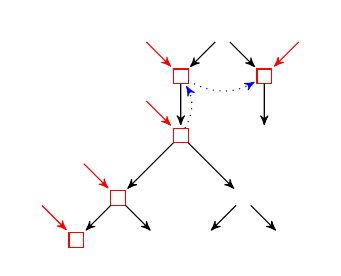
\begin{tikzpicture}[node distance=1cm,bend angle=30,transform shape,scale=0.75]
	    \node (1) {};     
	    \node[below left of=1] (2) {};    
	    \node[below of=2] (4) {};         
	    \node[below left of=4,node distance=1.5cm] (6) {};   
	    \node[below left of=6] (8) {};     
	    \node[below right of=6] (9) {};      
	    \node[below right of=4,node distance=1.5cm] (7) {};  
	    \node[below left of=7] (10) {};    
	    \node[below right of=7] (11) {};        
	    \node[below right of=1] (3) {};  
	    \node[below  of=3] (5) {};
\node[inner sep=0pt,draw, rectangle, fit=(6), color=red] (nu) {};
	    \node[above left of=nu,node distance=1cm,color=red] (nuet) {};
\node[inner sep=0pt,draw, rectangle, fit=(8), color=red] (nu0) {};
	    \node[above left of=nu0,node distance=1cm,color=red] (nu0et) {};
\node[inner sep=0pt,draw, rectangle, fit=(4), color=red] (nu1) {};
	    \node[above left of=nu1,node distance=1cm,color=red] (nu1et) {};
\node[inner sep=0pt,draw, rectangle, fit=(2), color=red] (nu2) {};
	    \node[above left of=nu2,node distance=1cm,color=red] (nu2et) {};
\node[inner sep=0pt,draw, rectangle, fit=(3), color=red] (nu3) {};
	    \node[above right of=nu3,node distance=1cm,color=red] (nu3et) {};
\path[->,color=red]
	      (nuet) edge (nu)
	      (nu0et) edge (nu0)
	      (nu1et) edge (nu1)
	      (nu2et) edge (nu2)
	      (nu3et) edge (nu3)
	    ;
	    \path[->,color=blue,dotted]
	      (4) edge[bend right] (2)
	      (2) edge[bend right] (3)
	    ;
	    \path[->]
	      (1) edge (2)
	      (1) edge (3)
	      (2) edge (4)
	      (3) edge (5)
	      (4) edge (6)
	      (4) edge (7)
	      (6) edge (8)
	      (6) edge (9)
	      (7) edge (10)
	      (7) edge (11)
	    ;
	  \end{tikzpicture}
	 }
	  \caption{ZPC-Structure of .}
	  \label{fig zpc e}
	\end{figure}
\end{minipage}

\noindent  A \emph{-Pseudo-Continuation}  of  in  is obtained from the 
 -C-Continuation  by replacing some subexpression  of  by a symbol  such that for two subexpressions 
  and  of :   
.


\begin{definition}\label{def2}
Let  be a regular expression over  and  be a bijection that associates to each subexpression of  a symbol in an alphabet . We define the word  over the alphabet  inductively as follows:
   
 \centerline{}
      
  \noindent The function  is said to be an -encoding.
\end{definition}

\begin{definition}
Let  and  be two integers such that ,  be a symbol in   and  an -encoding for some alphabet . The -Pseudo-Continuation of  in , denoted by , is the word over  defined by .
\end{definition}

In the following, we consider that the pseudo-continuations of 

are defined over  a finite subset of , bounded by the number of subexpressions of .

\begin{lemma}\label{lem egal psi egal exp}
  Let  and  be two regular expressions over an alphabet  such that  and  are two products of subexpressions of a regular expression  over . Let  be a -encoding. Then:
  
  \centerline{
      .
  }
\end{lemma}
\begin{proof}
  Let us consider that  is associated with the bijection . Let us consider the possible roots of the expressions.
  \begin{enumerate}
    \item If the roots of  and  are notconcatenation products,    since  is a bijection and .
  
    \item Let us suppose that, without loss of generality, only the root of  is aconcatenation product . Then the symbol  appears in  but not in . Hence  and .
  
    \item Finally, let us suppose that  and . 
    \begin{enumerate}
      \item If  then  and then  and  do not end with the same symbol.
      \item Suppose that . If ,  ends with  ; Hence  and . Otherwise, by induction hypothesis,   . Hence   .
    \end{enumerate}
  \end{enumerate}
  \qed
\end{proof}

\begin{proposition}\label{prop long pseudo cont lin}
The two following propositions hold:
  \begin{enumerate}
    \item  is at most linear w.r.t. ,
    \item  is at most linear w.r.t. , with . 
  \end{enumerate} 
\end{proposition}
  \begin{proof}
  
We define the function  as the number of 
left-associated
 concatenation operators
 in  as follows: 

\centerline{
    
  }
 


 Let us first prove that . The proof proceeds by induction in the structure of .

 \begin{enumerate} 
   \item Whenever  is not a product, . Hence . Since , the condition is satisfied.
\item Suppose that . Hence 

  \centerline{
    \begin{tabular}{l@{\ }l}
       & \\
      & \\
      & \\
      & .\\
    \end{tabular}
  }
  \end{enumerate}
 


Following Proposition~\ref{b},  where  is the node of  labelled by ,  is the ,  and for  such that . Since  are ancestors of , . Consequently, . Moreover, from previous point, . Consequently, .
  
  
 Furthermore, since , it holds:
 
 \centerline{.}
 
 However, the concatenation operators below the node  do not appears below another symbol. Consequently, 
 
 \centerline{}
 
 Finally,
 
 \centerline{.}
 
  \qed
 \end{proof}



\begin{proposition}\label{prop1}
Let , ,  and  be two integers. Then .
\end{proposition}
\begin{proof}
  Direct Corollary of Lemma~\ref{lem egal psi egal exp}.
 \qed
\end{proof}

  From Proposition~\ref{prop1} we can deduce that the -C-Continuations identification can be achieved by considering the -Pseudo-Continuations. In the following we show that this identification step (computation of ) can be done without the computation of the -Pseudo-Continuations and  that it amounts to the minimization of a word acyclic deterministic automaton. Before seeing how the identification of -Pseudo-Continuations  is performed, we prove that the computation of the function  can be done in a linear time in the size of . 

Let us consider the syntax tree  associated with 
.
 This syntax tree contains all the subexpressions of . Each node  in  corresponds to the 
subexpression  of . The equivalence relation  over the nodes of the tree  is defined by . We show that the computation of the equivalence relation  amounts to the minimization of the word acyclic deterministic automaton , where  is the node associated to the root of ,  with , , and  is defined by  if ,  and  if ,  if ,  if , and  in all otherwise. 

\begin{lemma}\label{lem exp egal si lang eq}
  .
\end{lemma} 
\begin{proof}
  Let  (resp. ) be the alphabet of the automaton  (resp. ).
  
  \begin{enumerate}
    \item If  then  and .
    \item Suppose that .  Notice that any word  in  (resp. ) starts with a symbol associated with the root of  (resp. ). 
    \begin{enumerate}
      \item Hence, if the roots of  and  are distinct, then  ; Since  is not empty by construction, . 
      \item Otherwise, there exists an integer  such that ,  and . By induction over the size of .
      \begin{enumerate}
        \item If , then since the roots are distincts, the word starting with the symbol associated to the node  followed by the symbol  is in  but not in .
        \item Otherwise, it holds by induction hypothesis that there exists a word in  not in . Hence there exists a word starting with a symbol associated to the node  followed by a word in  that is in  but not in .
      \end{enumerate}
    \end{enumerate}
  \end{enumerate}
  \qed
\end{proof}

 According to Lemma~\ref{lem exp egal si lang eq}, , that is the equivalence relation  coincides with Myhill-Nerode equivalence~\cite{Nerode} over the states of the automaton , that can be computed in  time and space complexity using Revuz Algorithm~\cite{revuz}.
 
\begin{lemma}\label{lemma5}
The computation of  for all subexpression  of  can be done in  time and space complexity.
\end{lemma}
\begin{proof}
  Let  and  be two nodes in . As , we can associate to each 
node  in  (each ) a symbol () which uniquely identifies its equivalence class . Furthermore, according to Lemma~\ref{lem exp egal si lang eq}, the computation of the equivalence relation  amounts to the minimization of the word acyclic deterministic automaton , which can be performed in  using Revuz Algorithm~\cite{revuz}. 
 \qed
\end{proof}

\noindent \begin{minipage}{0.45\linewidth}
  \begin{figure}[H]
	 \centerline{
	  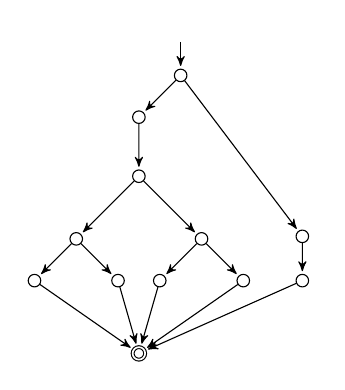
\begin{tikzpicture}[node distance=1cm,bend angle=30,transform shape,scale=0.75]
	    \node[state,initial above] (1) {};     
	    \node[state,below left of=1] (2) {};    
	    \node[state,below of=2] (4) {};         
	    \node[state,below left of=4,node distance=1.5cm] (6) {};   	    \node[state,below left of=6] (8) {};     
	    \node[state,below right of=6] (9) {};      
	    \node[state,below right of=4,node distance=1.5cm] (7) {};  	    \node[state,below left of=7] (10) {};    
	    \node[state,below right of=7] (11) {};  
	    \node[state,right of=11] (5) {};           
	    \node[state,above of=5,node distance=0.75cm] (3) {};
	    \node[accepting,state,below of=4,node distance=3cm] (12) {};        
	    \path[->]
	      (1) edge node[above left,pos=0.4] {} (2)
	      (1) edge node[above right,pos=0.4] {} (3)
	      (2) edge node[left,pos=0.4] {} (4)
	      (3) edge node[right,pos=0.4] {} (5)
	      (4) edge node[above left,pos=0.4] {} (6)
	      (4) edge node[above right,pos=0.4] {} (7)
	      (6) edge node[above left,pos=0.4] {} (8)
	      (6) edge node[above right,pos=0.4] {} (9)
	      (7) edge node[above left,pos=0.4] {} (10)
	      (7) edge node[above right,pos=0.4] {} (11)
	      (8) edge node[left,pos=0.4] {} (12)
	      (9) edge node[left,pos=0.4] {} (12)
	      (10) edge node[left,pos=0.4] {} (12)
	      (11) edge node[left,pos=0.4] {} (12)
	      (5) edge node[below right,pos=0.4] {} (12)
	    ;
	  \end{tikzpicture}
	 }
	  \caption{The automaton  .}
	  \label{fig a t e}
	\end{figure}
\end{minipage}
\hfill
\begin{minipage}{0.45\linewidth}
	\begin{figure}[H]
	 \centerline{
	  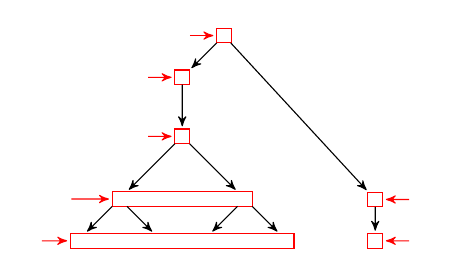
\begin{tikzpicture}[node distance=1cm,bend angle=30,transform shape,scale=0.75]
	    \node (1) {};     
	    \node[below left of=1] (2) {};    
	    \node[below of=2] (4) {};         
	    \node[below left of=4,node distance=1.5cm] (6) {};   
	    \node[below left of=6] (8) {};     
	    \node[below right of=6] (9) {};      
	    \node[below right of=4,node distance=1.5cm] (7) {};  
	    \node[below left of=7] (10) {};    
	    \node[below right of=7] (11) {};  
	    \node[right  of=11, node distance=1.5cm] (5) {};       
	    \node[above of=5,node distance=0.7cm] (3) {}; 
\node[inner sep=0pt,draw, rectangle, fit=(8)(11), color=red] (eq1) {};
	    \node[left of=eq1,node distance=2.5cm,color=red] (eq1et) {};
\node[inner sep=0pt,draw, rectangle, fit=(5), color=red] (eq2) {};
	    \node[right of=eq2,node distance=0.7cm,color=red] (eq2et) {};
\node[inner sep=0pt,draw, rectangle, fit=(6)(7), color=red] (eq3) {};
	    \node[left of=eq3,node distance=2cm,color=red] (eq3et) {};
\node[inner sep=0pt,draw, rectangle, fit=(3), color=red] (eq4) {};
	    \node[right of=eq4,node distance=0.7cm,color=red] (eq4et) {};
\node[inner sep=0pt,draw, rectangle, fit=(4), color=red] (eq5) {};
	    \node[left of=eq5,node distance=0.7cm,color=red] (eq5et) {};
\node[inner sep=0pt,draw, rectangle, fit=(2), color=red] (eq6) {};
	    \node[left of=eq6,node distance=0.7cm,color=red] (eq6et) {};
\node[inner sep=0pt,draw, rectangle, fit=(1), color=red] (eq7) {};
	    \node[left of=eq7,node distance=0.7cm,color=red] (eq7et) {};
\path[->,color=red]
	      (eq1et) edge (eq1)
	      (eq2et) edge (eq2)
	      (eq3et) edge (eq3)
	      (eq4et) edge (eq4)
	      (eq5et) edge (eq5)
	      (eq6et) edge (eq6)
	      (eq7et) edge (eq7)
	    ;
	    \path[->]
	      (1) edge (2)
	      (1) edge (3)
	      (2) edge (4)
	      (3) edge (5)
	      (4) edge (6)
	      (4) edge (7)
	      (6) edge (8)
	      (6) edge (9)
	      (7) edge (10)
	      (7) edge (11)
	    ;
	  \end{tikzpicture}
	 }
	  \caption{The Equivalence Classes.}
	  \label{fig es sim}
	\end{figure}
\end{minipage}


\begin{example}
  Let us consider the regular expression   of the Example~\ref{ex calc c cont}. Applying Myhill-Nerode equivalence~\cite{Nerode} to the states of the automaton  (Figure~\ref{fig a t e}) results in  equivalence classes labeled by . For example  and  (Figure~\ref{fig es sim}). Finally, . 
\end{example}

Recall that the -Pseudo-Continuation identification can be achieved in  \cite{ZPC2,automate2} using Paige and Tarjan's sorting algorithm~\cite{tarjan}. In what follows we show that this step amounts to the minimization of the acyclic deterministic word automaton  defined  with  and  by: 
\begin{itemize}
\item ,
\item ,
\item  is defined as follows:
	\begin{itemize}
	\item  for all  ,
	\item  if  is the  child of ,
	\item  if  and ,
	\item  and if  and  in all otherwise.  
	 \end{itemize}
\end{itemize}     

\begin{proposition}\label{prop lang B-T-E}

\end{proposition}
\begin{proof}
  By construction of , there exists a path from any state  with  and  to the root of  labelled by  where  is the node of  labelled by ,  is the ,  and for  such that . This word exactly corresponds to the word .
 \qed
\end{proof} 

Let  and  be two positions in .  As a direct consequence of Proposition~\ref{prop lang B-T-E},  if and only if the states  and  of  are equivalent. We eliminate the -transitions from the automaton . Since it has no -transitions cycles, this elimination can be performed in a linear time in the size of . Hence, we obtain a more compacted but equivalent structure, which we denote by .

\noindent \begin{minipage}{0.45\linewidth}
  \begin{figure}[H]
	 \centerline{
	  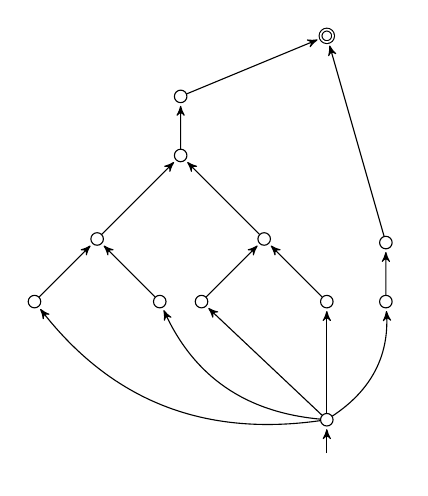
\begin{tikzpicture}[node distance=1cm,bend angle=30,transform shape,scale=0.75]
	    \node[state, initial below] (nut) {};  
	    \node[state, above of=nut,node distance=2cm] (f22) {};   	    \node[state, above left of=f22,node distance=1.5cm] (f2) {};  
	    \node[state, below left of=f2,node distance=1.5cm] (f21) {};   
	    \node[state, above left of=f2,node distance=2cm] (+) {}; 
	    \node[state, below left of=+,node distance=2cm] (f1) {}; 
	    \node[state, below right of=f1,node distance=1.5cm] (f12) {}; 
	    \node[state, below left of=f1,node distance=1.5cm] (f11) {}; 
	    \node[state, above of=+] (*a) {}; 
	    \node[state, above of=nut,accepting,node distance=6.5cm] (pa) {};  
	    \node[state, right of=f22] (h31) {}; 
	    \node[state, above of=h31] (h3) {}; 
	    \path[->]
	      (nut) edge node[right] {} (f22)
	      (nut) edge node[above right] {} (f21)
	      (nut) edge[bend left] node[below left] {} (f12)
	      (nut) edge[bend left] node[below left] {} (f11)
	      (nut) edge[bend right] node[right] {} (h31)
	      (h31) edge node[right] {} (h3)
	      (f22) edge node[above right] {} (f2)
	      (f21) edge node[above left] {} (f2)
	      (f12) edge node[above right] {} (f1)
	      (f11) edge node[above left] {} (f1)
	      (f1) edge node[above left] {} (+)
	      (f2) edge node[above right] {} (+)
	      (+) edge node[left] {} (*a)
	      (*a) edge node[above left] {} (pa)
	      (h3) edge node[right] {} (pa)
	    ;
	  \end{tikzpicture}
	 }
	  \caption{The automaton .}
	  \label{fig aut btbe}
	\end{figure}
\end{minipage}
\hfil
\begin{minipage}{0.45\linewidth}
  \begin{figure}[H]
	 \centerline{
	  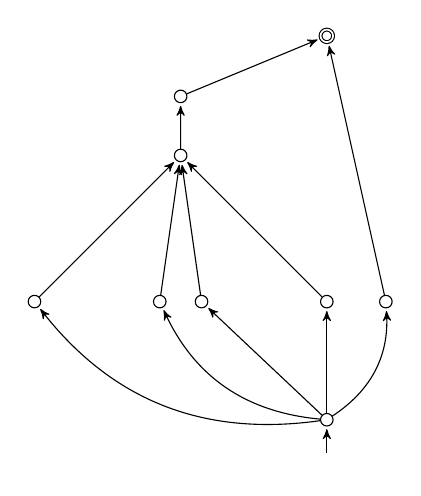
\begin{tikzpicture}[node distance=1cm,bend angle=30,transform shape,scale=0.75]
	    \node[state, initial below] (nut) {};  
	    \node[state, above of=nut,node distance=2cm] (f22) {};   	    \node[above left of=f22,node distance=1.5cm] (f2) {};  
	    \node[state, below left of=f2,node distance=1.5cm] (f21) {};   
	    \node[state, above left of=f2,node distance=2cm] (+) {}; 
	    \node[below left of=+,node distance=2cm] (f1) {}; 
	    \node[state, below right of=f1,node distance=1.5cm] (f12) {}; 
	    \node[state, below left of=f1,node distance=1.5cm] (f11) {}; 
	    \node[state, above of=+] (*a) {}; 
	    \node[state, above of=nut,accepting,node distance=6.5cm] (pa) {};  
	    \node[state, right of=f22] (h31) {}; 
	    \node[above of=h31] (h3) {}; 
	    \path[->]
	      (nut) edge node[right] {} (f22)
	      (nut) edge node[above right] {} (f21)
	      (nut) edge[bend left] node[below left] {} (f12)
	      (nut) edge[bend left] node[below left] {} (f11)
	      (nut) edge[bend right] node[right] {} (h31)
	      (h31) edge node[right] {} (pa)
	      (f22) edge node[above right] {} (+)
	      (f21) edge node[right] {} (+)
	      (f12) edge node[left] {} (+)
	      (f11) edge node[above left] {} (+)
	      (+) edge node[left] {} (*a)
	      (*a) edge node[above left] {} (pa)
	    ;
	  \end{tikzpicture}
	 }
	  \caption{The automaton .}
	  \label{fig aut eps free btbe}
	\end{figure}
\end{minipage}

The computation of the equivalence relation  can be performed by the computation of Myhill-Nerode relation~\cite{Nerode} on the states of the automaton . This automaton is deterministic and acyclic.

\begin{theorem}\label{theo sim e temps lin}
The  relation  can be computed in  time complexity.
\end{theorem}
\begin{proof}
 
 The equivalence relation  coincides with Myhill-Nerode equivalence~\cite{Nerode} on the states of the automaton 
 . 
 
 This automaton is deterministic and acyclic and its size is linear with respect to  (Proposition~\ref{prop long pseudo cont lin}). That can be computed in  time and space complexity using Revuz Algorithm~\cite{revuz}. 
  \qed
\end{proof}

\noindent \begin{minipage}{0.55\linewidth}
	\begin{example}
	  Let us consider the regular expression   of Example~\ref{ex calc c cont}.  The automaton  is represented by Figure~\ref{fig aut btbe}. The automaton  is represented in Figure~\ref{fig aut eps free btbe}. Applying Myhill-Nerode equivalence to the automaton  results in the automaton in Figure~\ref{fig min aut eps free btbe}. We deduce from this automaton that . Consequently the set of states of  is .
	\end{example}
\end{minipage}
\hfill
\begin{minipage}{0.4\linewidth}
  \begin{figure}[H]
	 \centerline{
	  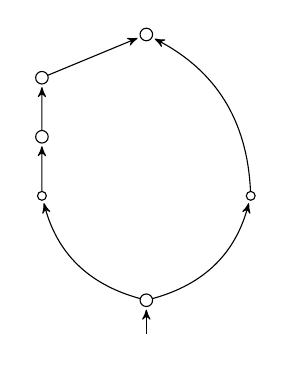
\begin{tikzpicture}[node distance=1cm,bend angle=30,transform shape,scale=0.75]
	    \node[state, initial below] (nut) {};
	    \node[state, above left of=nut,rounded rectangle,node distance=2.5cm] (f) {};
	    \node[state, above of=f] (+) {};
	    \node[state, above of=+] (*a) {};
	    \node[state, above of=nut, node distance=4.5cm] (pa) {};
	    \node[state, above right of=nut,rounded rectangle,node distance=2.5cm] (h) {};
\path[->]
	      (nut) edge[bend left] node[below left] {} (f)
	      (nut) edge[bend right] node[below right] {} (h)
	      (f) edge node[left] {} (+)
	      (+) edge node[left] {} (*a)
	      (*a) edge node[above left] {} (pa)
	      (h) edge[bend right] node[above right] {} (pa)
	    ;
	  \end{tikzpicture}
	 }
	  \caption{The Minimal Automaton of .}
	  \label{fig min aut eps free btbe}
	\end{figure}
\end{minipage}

\subsection{Computation of the set of transition rules}

Using Proposition~\ref{prop2} and Proposition\ref{prop equiv g-1 first}, we can show that the computation of the set of transitions of the equation tree automaton is performed by computing the function . The computation of a transition rule using Proposition~\ref{prop2} requires a linear time, according to Proposition~\ref{prop tps lin pour follow}. Then for all transition rules we get an  time and space complexity where  is the set of C-Continuations of . 
The computation of the set of states  make possible the creation of non-coaccessible states. Removing these states requires an  time complexity.

\begin{theorem}\label{theo eq tps cons}
 The equation tree automaton  of   can be computed in  time and space complexity with  the set of states of  . 
\end{theorem}
\begin{proof}
  The equivalence relation  can be computed in  time and space complexity and the set of transition rules can be performed by 
  computing the function . The computation of a transition rule using Proposition~\ref{prop2} requires a linear time, according 
  to Proposition~\ref{prop tps lin pour follow}. Then for all transition rules we get an  time and 
  space complexity where  is the set of C-Continuations of . Finally, removing not coaccessible states can be performed in linear time and results in the equation automaton.
  \qed
\end{proof}
\section{A Full Example}\label{sec:exemple}
Let  be a regular expression defined over the ranked alphabet  
such that , ,  and  be its linearized form.

The computation of the -C-Continuations of the  using the Definition~\ref{def1} is given in Table~\ref{tab c-cont}.

\begin{table}[H]
\centerline{
    \begin{tabular}{l@{\ }l}
	     & ,\\
	     & , \\
	     & ,\\
		 & ,\\ 
		 & ,\\    
		 & ,\\  
		 & ,\\ 
		 & ,\\ 
		 & .
   \end{tabular}
  }
  \caption{The -C-Continuations of .}
  \label{tab c-cont}
\end{table}

From Table~\ref{tab c-cont}, the Follow function can be computed (Table~\ref{tabl folow}).

\begin{minipage}{0.4\linewidth}
\begin{table}[H]
  \centerline{
    \begin{tabular}{|@{\ }c@{\ }|@{\ }c@{\ }|}
      \hline
       & \\
      \hline
       & \\
       & \\
       & \\
       & \\
       & \\
       & \\
       & \\
       & \\
       & \\
      \hline
    \end{tabular}
  }
  \caption{The function Follow.}
  \label{tabl folow}
\end{table}
\end{minipage}
\hfill
\begin{minipage}{0.55\linewidth}
 \begin{figure}[H] 
	 \centerline{
	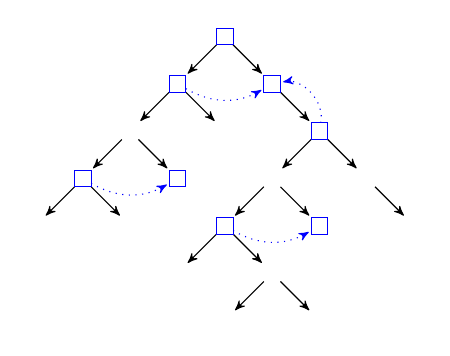
\begin{tikzpicture}[node distance=1cm,bend angle=30,transform shape,scale=0.85]
		\node[above] (1) {};
		\node[below left of=1] (2) {}; 
		\node[below right of=1] (3) {}; 
		\node[below right of=2] (4) {};
		\node[below left of=2] (5) {};
		\node[below right of=5] (16) {};
		\node[below left of=5] (17) {};
		\node[below left of=17] (18) {}; 
        \node[below right of=17] (19) {};
		\node[below right of=3] (6) {};
		\node[below right of=6] (7) {}; \node[below right of=7] (9) {};
	\node[below left of=6] (8) {}; \node[below right of=8](11){};
	 \node[below left of=8] (10) {};  \node[below left of=10] (12) {}; 
	 \node[below right of=10] (13) {}; \node[below left of=13] (14) {}; 
	 \node[below right of=13] (15) {};
	 \path[->]
	      (1) edge node[above left,pos=0.4] {} (2)
	      (1) edge node[above right,pos=0.4] {} (3)
	      (2) edge node[left,pos=0.4] {} (4)
	      (2) edge node[left,pos=0.4] {} (5)
	      (3) edge node[right,pos=0.4] {} (6)
	      (5) edge node[above left,pos=0.4] {} (16)
	      (5) edge node[above left,pos=0.4] {} (17)
	      (6) edge node[above left,pos=0.4] {} (7)
	      (6) edge node[above right,pos=0.4] {} (8)
	      (7) edge node[above right,pos=0.4] {} (9)
	      (8) edge node[above left,pos=0.4] {} (10)
	      (8) edge node[above right,pos=0.4]{} (11)
	      (10) edge node[above right,pos=0.4] {} (12)
	      (10) edge node[above left,pos=0.4] {} (13)
	      (13) edge node[above right,pos=0.4] {} (14)
	      (13) edge node[above left,pos=0.4] {} (15)
	      (17) edge node[left,pos=0.4] {} (18)
	      (17) edge node[left,pos=0.4] {} (19)
	     ;
	      \path[->,color=blue,dotted]
	      (17) edge[bend right] (16)
	      (2) edge[bend right] (3)
	      (10) edge[bend right] (11)
	      (6) edge[bend right=55] (3)
	    ;
	     \node[inner sep=0pt,draw, fit=(1), color=blue] (eq1) {};
	    \node[left of=eq1,node distance=0.5cm,color=blue] (eq1et) {};
	     \node[inner sep=0pt,draw, fit=(2), color=blue] (eq2) {};
	    \node[left of=eq2,node distance=0.5cm,color=blue] (eq2et) {};
	      \node[inner sep=0pt,draw, fit=(17), color=blue] (eq3) {};
	    \node[left of=eq3,node distance=0.5cm,color=blue] (eq3et) {};	    
	    \node[inner sep=0pt,draw, fit=(16), color=blue] (eq8) {};
	    \node[left of=eq8,node distance=0.5cm,color=blue] (eq8et) {};
	     \node[inner sep=0pt,draw, fit=(3), color=blue] (eq4) {};
	      \node[left of=eq4,node distance=0.5cm,color=blue] (eq4et) {};
	     \node[inner sep=0pt,draw, fit=(6), color=blue] (eq6) {};
	    \node[left of=eq6,node distance=0.5cm,color=blue] (eq6et) {};
	     \node[inner sep=0pt,draw, fit=(10), color=blue] (eq5) {};
	    \node[left of=eq5,node distance=0.5cm,color=blue] (eq5et) {};
	    \node[inner sep=0pt,draw, fit=(11), color=blue] (eq7) {};
	    \node[left of=eq7,node distance=0.5cm,color=blue] (eq7et) {};
	 \end{tikzpicture}
	 }
	  \caption{The ZPC-Structure of .}\label{fig a t e1}
	\end{figure}
\end{minipage}

Finally, from Table~\ref{tabl folow}, the transition function of   is the following:

\centerline{
  \begin{tabular}{r@{\ }c@{\ }l@{\ \ \ \ \ \ \ }r@{\ }c@{\ }l}
     &  &  &  &  & \\
     &  &  &  &  & \\
     &  &  &  &  & \\
      &  &  &  &  & \\
     &  &  &  &  & \\
     &  &  &  &  & \\
  \end{tabular}
}

  The ZPC-structure associated to  is represented in Figure~\ref{fig a t e1}. The dotted links in Figure~\ref{fig a t e1} represent the function :

\centerline{
  , , , .
  }
 
The automaton  associated with  is  represented in Figure~\ref{fig a t e2}. 
 
 \begin{figure}[H] 
	 \centerline{
		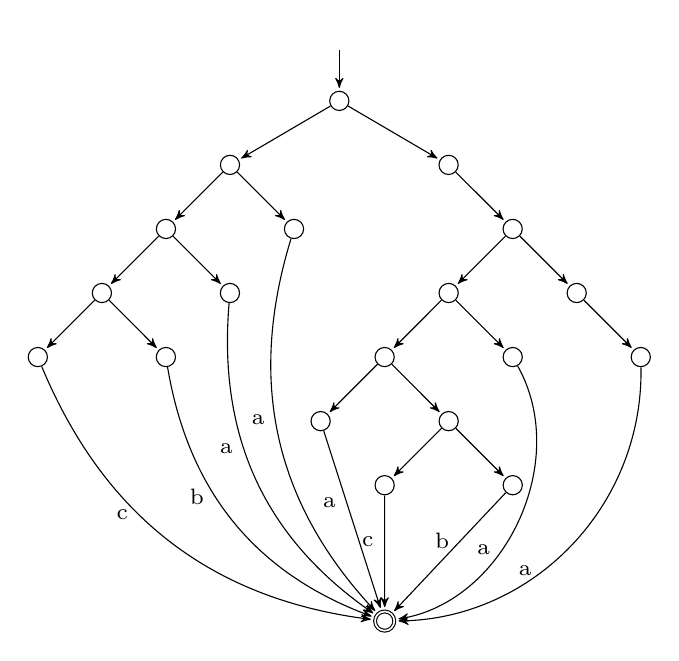
\begin{tikzpicture}[node distance=1cm,bend angle=30,transform shape,scale=1.15]
\node[state,initial above] (1) {};
		\node[state,below left of=1,xshift=-5mm] (2) {}; 
		\node[state,below right of=1,xshift=5mm] (3) {}; 
		\node[state,below right of=2] (4) {};
		\node[state,below left of=2] (5) {};
		\node[state,below right of=5] (16) {};
		\node[state,below left of=5] (17) {};
		\node[state,below left of=17] (18) {}; 
	 \node[state,below right of=17] (19) {};
		\node[state,below right of=3] (6) {};
		\node[state,below right of=6] (7) {}; \node[state,below right of=7] (9) {};
	\node[state,below left of=6] (8) {}; \node[state,below right of=8](11){};
	 \node[state,below left of=8] (10) {};  \node[state,below left of=10] (12) {}; 
	 \node[state,below right of=10] (13) {}; \node[state,below left of=13] (14) {}; 
	 \node[state,below right of=13] (15) {};
	 \node[accepting,state,below of=14,node distance=1.5cm] (20) {};
	 \path[->]
	      (1) edge node[above left,pos=0.4] {} (2)
	      (1) edge node[above right,pos=0.4] {} (3)
	      (2) edge node[right,pos=0.1] {} (4)
	      (2) edge node[left,pos=0.1] {} (5)
	      (3) edge node[right,pos=0.1] {} (6)
	      (5) edge node[above right,pos=0.4] {} (16)
	      (5) edge node[above left,pos=0.4] {} (17)
	      (6) edge node[above right,pos=0.4] {} (7)
	      (6) edge node[above left ,pos=0.4] {} (8)
	      (7) edge node[above right,pos=0.4] {} (9)
	      (8) edge node[above left,pos=0.6] {} (10)
	      (8) edge node[above right,pos=0.6]{} (11)
	      (10) edge node[above left,pos=0.4] {} (12)
	      (10) edge node[above right,pos=0.4] {} (13)
	      (13) edge node[above left,pos=0.4] {} (14)
	      (13) edge node[above right,pos=0.4] {} (15)
	      (17) edge node[left,pos=0.1] {} (18)
	      (17) edge node[right,pos=0.1] {} (19)
(4) edge [bend right]node[left,pos=0.45] {a} (20)
	      (9) edge [bend left=45] node[left,pos=0.6] {a} (20) 
	      (11) edge [bend left=55]node[left,pos=0.6] {a} (20)
	      (12) edge node[left,pos=0.4] {a} (20)
	      (14) edge node[left,pos=0.4] {c} (20)
	      (15) edge node[left,pos=0.4] {b} (20)
	      (16) edge [bend right]node[left,pos=0.4] {a} (20)
	      (18) edge [bend right]node[left,pos=0.4] {c} (20)
	      (19) edge [bend right]node[left,pos=0.4] {b} (20)	      
	     ;
	 \end{tikzpicture}
	 }
	  \caption{The automaton .}
	  \label{fig a t e2}
	\end{figure}	
Applying Myhill-Nerode equivalence relation over the states of the automaton  results in the automaton in Figure~\ref{fig a t e3}.


 \begin{figure}[H] 
	 \centerline{
		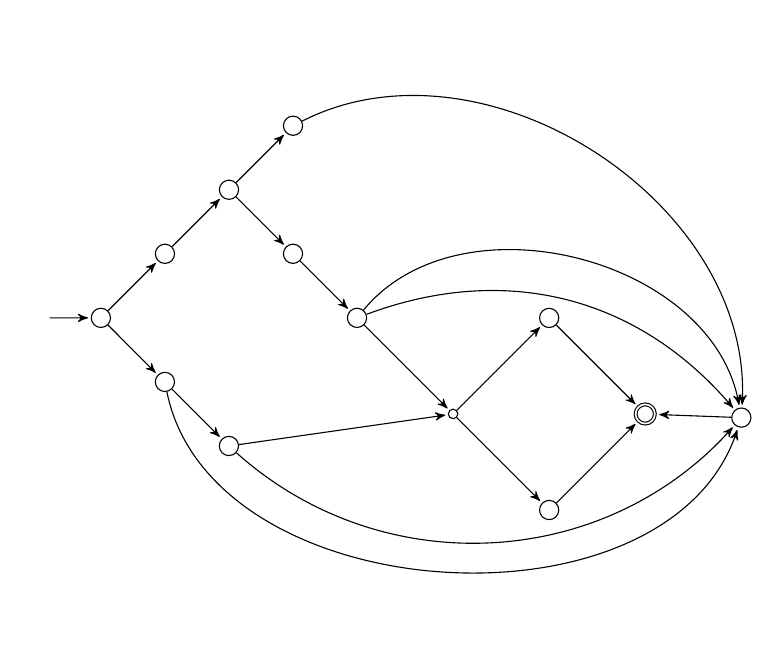
\begin{tikzpicture}[node distance=1cm,bend angle=50,transform shape,scale=1.15]
\node[state,above] (1) {};
		\node[state,below left of=1] (2) {}; 
		\node[state,below left of=2] (3) {}; 
		\node[state,below right of=2](4) {}; 
		\node[initial, state,below left of=3] (5) {};
		\node[state,below right of=5](6) {};		
		\node[state,below right of=6](7) {};
		\node[state,below right of=4](8) {};
		\node[state,below right of=8,node distance=1.5cm,scale=0.7,rounded rectangle] (9) {};
		\node[state,above right of=9,node distance=1.5cm] (10) {}; 
		\node[state,below right of=9,node distance=1.5cm](11) {}; 
     	\node[accepting,state,below right of=10,node distance=1.5cm] (12) {};
		\node[state,above right of=12,node distance=1.5cm,yshift=-11mm] (13) {};
	 \path[->]
	     (5) edge node[above left,pos=0.4] {} (3)
         (3) edge node[above left] {} (2)	     
	     (2) edge node[below right,pos=0.4] {} (1)
	     (2) edge node[below left,pos=0.4] {} (4)
         (4) edge node[below left,pos=0.4] {} (8)
         (8) edge node[below left,pos=0.4] {} (9)
	     (5) edge node[below left,pos=0.4] {} (6)
	     (6) edge node[above right,pos=0.4] {} (7)
	     (7) edge node[above left,pos=0.4] {} (9)
	     (9) edge node[above left,pos=0.4] {} (10)
	     (9) edge node[below left,pos=0.4] {} (11)
	      (10) edge node[below left,pos=0.4] {} (12)
	      (11) edge node[above left,pos=0.4] {} (12)
	      (13) edge node[above left,pos=0.4] {} (12)
	      (1) edge [bend left=60] node[right,pos=0.8] {} (13)
	      (8) edge [bend left=65] node[right,pos=0.6] {} (13)
    	      (8) edge [bend left=35] node[right,pos=0.7] {} (13)
    	      (7) edge [bend right=45] node[left,pos=0.2] {} (13)
    	      (6) edge [bend right=75] node[left,pos=0.18] {} (13)	      
	     ;
	 \end{tikzpicture}
	 }
	  \caption{The minimal automaton of .}
	  \label{fig a t e3}
	\end{figure}	
The computation of the equivalence relation  over the syntax tree associated to  is represented in the Figure~\ref{fig a t e4}. The number of equivalence classes in Figure~\ref{fig a t e4} () corresponds exactly to the number of states of the minimal automaton of . From these equivalence classes, we can define the  function (see Table~\ref{table psi}).  
	
	\begin{minipage}{0.40\linewidth}
	\begin{table}[H]
	  \centerline{
	    \begin{tabular}{l@{\ }l}
	       & \\
	       & \\
	       & \\
	       & \\
	       & \\
	       & \\
	       & \\
	       & \\
	       & \\
	       & \\
	       & \\
	       & \\
	    \end{tabular}
	  }
	  \caption{The function .}
	  \label{table psi}
	\end{table}
	\end{minipage}
	\hfill
	\begin{minipage}{0.55\linewidth}
	\begin{figure}[H] 
	 \centerline{
	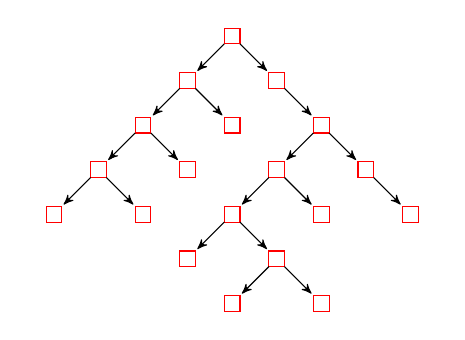
\begin{tikzpicture}[node distance=1cm,bend angle=30,transform shape,scale=0.8]
		\node(1) {};
		\node[below left of=1] (2) {}; 
		\node[below right of=1] (3) {}; 
		\node[below right of=2] (4) {};
		\node[below left of=2] (5) {};
		\node[below right of=5] (16) {};
		\node[below left of=5] (17) {};
		\node[below left of=17] (18) {}; 
	 \node[below right of=17] (19) {};
		\node[below right of=3] (6) {};
		\node[below right of=6] (7) {}; \node[below right of=7] (9) {};
	\node[below left of=6] (8) {}; \node[below right of=8](11){};
	 \node[below left of=8] (10) {};  \node[below left of=10] (12) {}; 
	 \node[below right of=10] (13) {}; \node[below left of=13] (14) {}; 
	 \node[below right of=13] (15) {};	 
	 \node[inner sep=0pt,draw, rectangle, fit=(1), color=red] (eq1) {};
	    \node[left of=eq1,node distance=0.5cm,color=red] (eq1et) {};
	    \node[inner sep=0pt,draw, rectangle, fit=(2), color=red] (eq2) {};
	    \node[left of=eq2,node distance=0.5cm,color=red] (eq2et) {};
	    \node[inner sep=0pt,draw, rectangle, fit=(3), color=red] (eq3) {};
	    \node[right of=eq3,node distance=0.5cm,color=red] (eq3et) {};
	    \node[inner sep=0pt,draw, rectangle, fit=(5), color=red] (eq4) {};
	    \node[left of=eq4,node distance=0.4cm,color=red] (eq4et) {};
	    \node[inner sep=0pt,draw, rectangle, fit=(4), color=red] (eq5) {};
	    \node[right of=eq5,node distance=0.3cm,color=red] (eq5et) {};
	    \node[inner sep=0pt,draw, rectangle, fit=(16), color=red] (eq6) {};
	    \node[right of=eq6,node distance=0.3cm,color=red] (eq6et) {};
	    \node[inner sep=0pt,draw, rectangle, fit=(19), color=red] (eq7) {};
	    \node[right of=eq7,node distance=0.3cm,color=red] (eq7et) {};
	    \node[inner sep=0pt,draw, rectangle, fit=(18), color=red] (eq8) {};
	    \node[left of=eq8,node distance=0.3cm,color=red] (eq8et) {};	
	    \node[inner sep=0pt,draw, rectangle, fit=(17), color=red] (eq9) {};
	    \node[left of=eq9,node distance=0.5cm,color=red] (eq9et) {};    
	    \node[inner sep=0pt,draw, rectangle, fit=(6), color=red] (eq10) {};
	   \node[right of=eq10,node distance=0.5cm,color=red] (eq10et) {};
	   \node[inner sep=0pt,draw, rectangle, fit=(7), color=red] (eq11) {};
	   \node[right of=eq11,node distance=0.5cm,color=red] (eq11et) {};
	   \node[inner sep=0pt,draw, rectangle, fit=(9), color=red] (eq12) {};
	   \node[right of=eq12,node distance=0.3cm,color=red] (eq12et) {};
	   \node[inner sep=0pt,draw, rectangle, fit=(11), color=red] (eq13) {};
	   \node[right of=eq13,node distance=0.3cm,color=red] (eq13et) {};
	   \node[inner sep=0pt,draw, rectangle, fit=(15), color=red] (eq14) {};
	   \node[right of=eq14,node distance=0.3cm,color=red] (eq14et) {};
	   \node[inner sep=0pt,draw, rectangle, fit=(12), color=red] (eq15) {};
	   \node[left of=eq15,node distance=0.3cm,color=red] (eq15et) {};
	   \node[inner sep=0pt,draw, rectangle, fit=(14), color=red] (eq16) {};
	   \node[left of=eq16,node distance=0.3cm,color=red] (eq16et) {};
	   \node[inner sep=0pt,draw, rectangle, fit=(8), color=red] (eq17) {};
	   \node[left of=eq17,node distance=0.5cm,color=red] (eq17et) {};
	   \node[inner sep=0pt,draw, rectangle, fit=(10), color=red] (eq18) {};
	   \node[left of=eq18,node distance=0.4cm,color=red] (eq18et) {};
	   \node[inner sep=0pt,draw, rectangle, fit=(13), color=red] (eq19) {};
	   \node[right of=eq19,node distance=0.4cm,color=red] (eq19et) {};
	 \path[->]
	      (1) edge node[above left,pos=0.4] {} (2)
	      (1) edge node[above right,pos=0.4] {} (3)
	      (2) edge node[left,pos=0.4] {} (4)
	      (2) edge node[left,pos=0.4] {} (5)
	      (3) edge node[right,pos=0.4] {} (6)
	      (5) edge node[above left,pos=0.4] {} (16)
	      (5) edge node[above left,pos=0.4] {} (17)
	      (6) edge node[above left,pos=0.4] {} (7)
	      (6) edge node[above right,pos=0.4] {} (8)
	      (7) edge node[above right,pos=0.4] {} (9)
	      (8) edge node[above left,pos=0.4] {} (10)
	      (8) edge node[above right,pos=0.4]{} (11)
	      (10) edge node[above right,pos=0.4] {} (12)
	      (10) edge node[above left,pos=0.4] {} (13)
	      (13) edge node[above right,pos=0.4] {} (14)
	      (13) edge node[above left,pos=0.4] {} (15)
	      (17) edge node[left,pos=0.4] {} (18)
	      (17) edge node[left,pos=0.4] {} (19)
	     ;
	 \end{tikzpicture}
	 }
	  \caption{The equivalence classes.}
	  \label{fig a t e4}
	\end{figure}
	\end{minipage}
	
	As we have seen, the computation of the equivalence relation  turns in the minimization of an acyclic deterministic automaton. The automaton  associated with  is represented in Figure~\ref{fig a t e5}. 
	\begin{figure}[H]	
	 \centerline{
	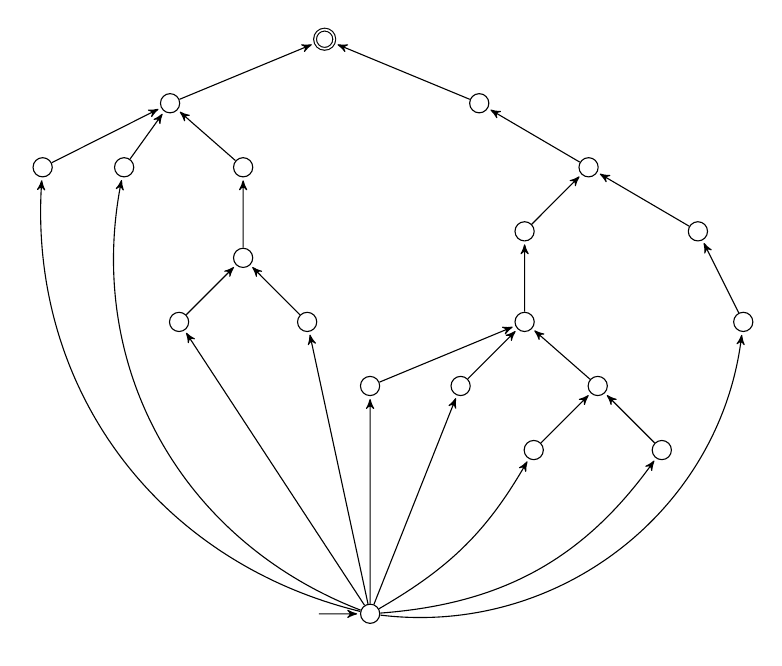
\begin{tikzpicture}[node distance=1cm,bend angle=30,transform shape,scale=1.15]	
	\node[accepting,state, above] (1) {};
	\node[state,below left of=1,xshift=-10mm] (2) {}; 
		\node[state,below right of=1,xshift=10mm] (3) {};
		\node[state,below right of=2,xshift=1mm] (5) {};
		\node[state,below left of=2,xshift=-7mm] (7) {};
		\node[state,below left of=2,xshift=2mm] (8) {};
		\node[state,below right of=3,xshift=5mm] (6) {};
		\node[state,below of=5] (9) {}; 
		\node[state,below left of=9] (10) {}; 
		\node[state,below right of=9] (11) {};
		\node[state,below left of=6] (12) {}; 
		\node[state,below of=12] (15) {};	
		\node[state,below right of=6,xshift=5mm] (13) {};	
		\node[state,below of=13,xshift=5mm] (14) {};	
		\node[state,below right of=15,xshift=1mm] (16) {};
		\node[state,below left of=15,xshift=-10mm] (17) {};
		\node[state,below left of=15] (18) {};
		\node[state,below left of=16] (19) {}; 
		\node[state,below right of=16] (20) {};
		\node[state,initial,below left of=19,xshift=-11mm,yshift=-11mm] (21) {}; 
		\path[->]
	      (2) edge node[above left,pos=0.4] {} (1)
	      (3) edge node[above right,pos=0.4] {} (1)
	      (5) edge node[above right] {} (2)
	      (8) edge node[right,pos=-0.1] {} (2)
	      (7) edge node[above left] {} (2)
	      (6) edge node[above right,pos=0.4] {} (3)
	       (13) edge node[above right,pos=0.4] {} (6)
	        (14) edge node[above right,pos=0.4] {} (13)
	        (12) edge node[above left,pos=0.4] {} (6)
	        (15) edge node[above left,pos=0.1] {} (12)
	        (16) edge node[above right,pos=0.4] {} (15)
	        (17) edge node[above right,pos=0.2] {} (15)
	        (18) edge node[above right,pos=-0.6] {} (15)
	        (9) edge node[above right,pos=-0.1] {} (5)
	         (10) edge node[above left,pos=0.1] {} (9)
	          (11) edge node[above right,pos=0.1] {} (9)
	     	(19) edge node[above left,pos=0.1] {} (16)
	          (20) edge node[above right,pos=0.1] {} (16)
(21) edge [bend left=40]node[left,pos=0.45] {} (7)
	      (21) edge [bend left=40]node[left,pos=0.55] {} (8)
	      (21) edge node[left,pos=0.45] {} (10)
	      (21) edge node[left,pos=0.6] {} (11) 
	       (21) edge node[right,pos=0.5] {} (17)
	      (21) edge node[right,pos=0.5] {} (18) 
	      (21) edge [bend right=15] node[right,pos=0.5] {} (19)
	      (21) edge [bend right=25] node[right,pos=0.7] {} (20) 
	      	      (21) edge [bend right=45] node[right,pos=0.5] {} (14) 	          
	     ;
	 \end{tikzpicture}
	 }
	  \caption{The automaton .}
	  \label{fig a t e5}
	\end{figure}	
We eliminate the -transitions from the automaton . Since this last has no -transitions cycles, this elimination can be performed in a linear time in the size of . Hence, we obtain a structure which we denote .  
	\begin{figure}[H]	
	 \centerline{
	\begin{tikzpicture}[node distance=1cm,bend angle=30,transform shape,scale=1.15]	
	\node[accepting,state, above] (1) {};
	\node[state,below left of=1,xshift=-10mm] (2) {}; 
\node[state,below left of=2,xshift=-7mm] (7) {};
		\node[state,below left of=2,xshift=2mm] (8) {};
		\node[state,below right of=3,xshift=5mm] (6) {};
		\node[state,below of=5] (9) {}; 
		\node[state,below left of=9] (10) {}; 
		\node[state,below right of=9] (11) {};
\node[state,below of=12] (15) {};	
\node[state,below of=13,xshift=5mm] (14) {};	
\node[state,below left of=15,xshift=-10mm] (17) {};
		\node[state,below left of=15] (18) {};
		\node[state,below left of=16] (19) {}; 
		\node[state,below right of=16] (20) {};
		\node[state,initial,below left of=19,xshift=-11mm,yshift=-11mm] (21) {}; 
		\path[->]
	      (2) edge node[above left,pos=0.4] {} (1)
(8) edge node[right,pos=-0.1] {} (2)
	      (7) edge node[above left] {} (2)
	      (6) edge node[above right,pos=0.4] {} (1)
(14) edge node[above right,pos=0.4] {} (6)
(15) edge node[above left,pos=0.4] {} (6)
(17) edge node[above right,pos=0.2] {} (15)
	        (18) edge node[above right,pos=-0.6] {} (15)
	        (9) edge node[above right,pos=0.4] {} (2)
	         (10) edge node[above left,pos=0.1] {} (9)
	          (11) edge node[above right,pos=0.1] {} (9)
	     	(19) edge node[above right,pos=0.1] {} (15)
	          (20) edge node[above right,pos=0.1] {} (15)
(21) edge [bend left=40]node[left,pos=0.45] {} (7)
	      (21) edge [bend left=40]node[left,pos=0.55] {} (8)
	      (21) edge node[left,pos=0.45] {} (10)
	      (21) edge node[left,pos=0.6] {} (11) 
	       (21) edge node[right,pos=0.5] {} (17)
	      (21) edge node[right,pos=0.5] {} (18) 
	      (21) edge [bend right=15] node[right,pos=0.5] {} (19)
	      (21) edge [bend right=25] node[right,pos=0.7] {} (20) 
	      	      (21) edge [bend right=45] node[right,pos=0.5] {} (14) 	          
	     ;
	 \end{tikzpicture}
	 }
	  \caption{The automaton .}
	  \label{fig a t e6}
	\end{figure}
  
  
	The computation of the equivalence relation  amounts to apply Myhill-Nerode relation on the states of the automaton . The result is represented in Figure~\ref{fig a t e7}.
\begin{figure}[H]	
	 \centerline{
	\begin{tikzpicture}[node distance=2.5cm,bend angle=30,transform shape,scale=1.15]	
    \node[state, above of=1,rounded rectangle,node distance=1.5cm,] (9) {};	
	\node[state, above] (1) {};
	\node[initial,state,left of=1] (2) {}; 
	\node[state, below of=1,rounded rectangle,node distance=1.5cm,] (3) {};
	\node[state, below of=3,rounded rectangle,node distance=1.5cm,] (4) {};
	\node[state, below of=4,rounded rectangle,node distance=1.5cm,] (5) {};
	\node[state, right of=1,rounded rectangle] (6) {};
	\node[state, right of=6,rounded rectangle] (7) {};
	\node[accepting,state,right of=7] (8) {}; 
		\path[->]
	      (2) edge node[above left,pos=0.8] {} (9)
	      (2) edge node[above left,pos=0.98] {} (1)
	      (1) edge node[above right,pos=0.3] {} (6)
	      (2) edge node[above right] {} (3)
	      (2) edge node[ right,pos=0.75] {} (4)
	      (2) edge node[below left,pos=0.4] {} (5)	
	      (3) edge node[above ] {} (6)
	      (4) edge node[below right,pos=0.5] {} (6) 
	      (6) edge node[above left,pos=0.7] {} (7) 
	      (9) edge node[above right,pos=0.7] {} (7)
	      (5) edge node[below] {} (7) 
	      (7) edge node[above left,pos=0.9] {} (8)      	          
	     ;
	 \end{tikzpicture}
	 }
	  \caption{The Minimal Automaton of .}
	  \label{fig a t e7}
	\end{figure}		



The language recognized by  is the following:

\centerline{
  \begin{tabular}{l@{\ }l@{\ }l}
     & & \\
    &  & \\
    &  & \\
    &  & \\
    &  & \\
  \end{tabular}
}
Let us notice that Proposition~\ref{prop1} is satisfied in Table~\ref{tab lang ccont}. 
	
	
	\begin{table}[H]
	\centerline{ 
 \begin{tabular}{|@{\ }c@{\ }|@{\ }c@{\ }|@{\ }c@{\ }|}
   \hline
    &  & \\
   \hline
    &  & \\
    &  &  \\
    &  &  \\
    &  & \\
    &  & \\
    &  & \\
    &  & \\ 
    &  & \\
    &  & \\ 
   \hline
   \end{tabular}
  }
    \caption{ and -C-Continuations.}
    \label{tab lang ccont}
  \end{table}

  Finally, the equation automaton  associated with  is obtained from merging the states and the transitions using . The transition function is:
  
  \centerline{ 
  \begin{tabular}{r@{\ }c@{\ }l}
     &  & \\
     &  & \\
      &  & \\
      &  & \\
     &  & \\
     &  & \\
      &  & \\
  \end{tabular}
}

\section{Conclusion}

We presented a new and more efficient algorithm for the computation of the equation tree automaton from a regular tree expression by extending the notion of -c-continuation from words to trees. We proved that a regular tree expression  can be converted into an equation tree automaton with an  time and space complexity 
where  is the set of -C-Continuations of .

\bibliographystyle{splncs_srt}
\bibliography{bibliograph}


\end{document}
